\documentclass[conference,a4paper]{IEEEtran}
\usepackage{amsmath,amssymb}
\usepackage{graphicx}
\usepackage{array}
\usepackage{url}
\usepackage[colorlinks=true,linkcolor=black,citecolor=black,urlcolor=black]{hyperref}
\hyphenation{GARCH}

\renewcommand{\arraystretch}{1.08}
\setlength{\tabcolsep}{3.2pt}

\newcommand{\volf}{\sigma^{\mathrm{fwd}}}

\begin{document}

\title{Predicting Portfolio Risk with Machine Learning: A Walk-Forward Comparison Against GARCH-Type Baselines on Indian Equities and ETFs}

% --- placeholders: replace before submission ---------------------------------------------
\author{\IEEEauthorblockN{[Author 1]\IEEEauthorrefmark{1}, [Author 2]\IEEEauthorrefmark{1},
[Author 3]\IEEEauthorrefmark{1}, [Author 4]\IEEEauthorrefmark{1}}
\IEEEauthorblockA{\IEEEauthorrefmark{1}Department of [Department], Manipal Institute of Technology, Manipal, India\\
Minor Specialization Mini Project. Mentor: [Mentor name]\\
Emails: [author emails]}}

\maketitle

\begin{abstract}
We ask whether machine learning predicts the risk of a user-defined portfolio
better than established econometric models. Using 45 liquid NSE stocks and ETFs (2010--2026), we
train Random Forest, XGBoost and a single-layer multi-task LSTM on 400 random portfolios and predict
three targets over a 21-trading-day horizon: realised volatility, the probability of a drawdown of
at least 5\%, and 95\% one-day Value-at-Risk. Every model and baseline (naive, EWMA, HAR, GARCH,
GJR-GARCH with $t$ errors, filtered historical simulation, simulated drawdown) is scored on identical
rows in a six-fold expanding-window walk-forward design with a 21-day purge and 80 held-out
portfolios, with Diebold-Mariano tests (Holm-corrected), a model confidence set and VaR backtests.
ML is competitive but not better: GJR-GARCH is best on the losses robust to a noisy volatility proxy
(QLIKE 0.281 vs.\ 0.299 for the best ML model), and no ML model significantly beats it after
correction, although XGBoost and the LSTM significantly beat naive volatility. The only clear gain
over the baselines is from combining forecasts (lowest RMSE, 0.0697) and from a simulation-based
drawdown model (Brier 0.2046). In a downstream test, sizing a portfolio from any of these forecasts
brings realised volatility to about 10--11\% against 19\% unscaled, but the models are not reliably
ranked. We report the evaluation, its limits and the leakage safeguards in full.
\end{abstract}

\begin{IEEEkeywords}
portfolio risk, volatility forecasting, Value-at-Risk, GARCH, LSTM, XGBoost, walk-forward validation
\end{IEEEkeywords}

\section{Introduction}
Investors rarely care about the expected return of a portfolio as much as about how bad it can get:
how volatile it will be next month, how likely a sizeable drawdown is, and how much it can lose on
a bad day. Traditional answers come from volatility models such as EWMA, GARCH and HAR, or from
historical Value-at-Risk (VaR). Machine learning (ML) offers flexible alternatives that can use many
inputs at once, and several studies report gains for volatility forecasting \cite{christensen2023}.
Yet the classic evidence is that a plain GARCH(1,1) is hard to beat out of sample for exchange rates,
while for stock returns only models with a leverage effect did better \cite{hansen2005}, and ML comparisons are often run on one asset, with random splits, or with a weak baseline.

This project builds and evaluates a portfolio risk predictor for Indian markets and exposes it in a
Streamlit dashboard where a user enters tickers and weights. We make three contributions.
\begin{enumerate}
\item \emph{A portfolio-level setup.} Models are trained on 400 random portfolios (3--15 assets) so
that one model serves any user portfolio, with features built from the portfolio return series and
market/macro variables.
\item \emph{A strict, shared evaluation.} All models and baselines go through the same code, folds
and metrics, with leakage tests, an H-day purge, held-out portfolios and multiple-testing control.
\item \emph{An honest result.} ML is competitive with strong econometric models but does not
significantly beat the best of them; we say where it helps (against naive volatility, in combination
with HAR and GARCH) and where it does not.
\end{enumerate}
We also add a downstream test, motivated by work that judges forecasts by their effect on portfolio
outcomes: does a better volatility forecast give a better volatility-targeted portfolio?

\section{Related Work}
\textbf{Volatility models.} ARCH-type models \cite{bollerslev1986} and the asymmetric GJR variant
\cite{glosten1993} describe volatility clustering and leverage effects. RiskMetrics' EWMA
\cite{riskmetrics1996} is a one-parameter special case, and the HAR model \cite{corsi2009} regresses
future volatility on daily, weekly and monthly averages. Hansen and Lunde \cite{hansen2005} found
no model that clearly beat GARCH(1,1) for exchange rates, but evidence that models with a leverage
effect beat it for stock returns.

\textbf{ML for risk.} Tree ensembles \cite{breiman2001,chen2016} and recurrent networks
\cite{hochreiter1997} have been applied to volatility and return forecasting
\cite{christensen2023,gu2020}. We follow the common recommendation to give ML the econometric
forecasts as inputs and to compare against them fairly.

\textbf{Evaluation.} Realised volatility is a noisy proxy, so only some losses (QLIKE, MSE on
variance) rank forecasts consistently \cite{patton2011}. Forecast comparison uses the
Diebold-Mariano test \cite{dm1995} with a small-sample correction \cite{hln1997}, Holm's
step-down correction \cite{holm1979} and the model confidence set \cite{hansen2011}. VaR is checked
with Kupiec's coverage test \cite{kupiec1995} and Christoffersen's independence test
\cite{christoffersen1998}, and expected shortfall with the joint FZ0 loss \cite{patton2019}, which rests on the elicitability
of the pair \cite{fissler2016}.
Quantile (pinball) loss follows Koenker and Bassett \cite{koenker1978}. Filtered historical
simulation \cite{barone1999} and online conformal calibration \cite{gibbs2021} supply a simulation
baseline and a coverage correction.

\textbf{Forecasts and portfolios.} Moreira and Muir \cite{moreira2017} show that scaling exposure
by inverse forecast variance can improve risk-adjusted returns. Our downstream test uses the same
idea only to ask whether the forecasts are useful for risk control, not to claim a trading strategy.

\section{Data and Problem Setup}
\subsection{Data}
The universe has 45 liquid NSE instruments: 40 large-cap stocks across IT, financials, energy,
consumer, auto, industrials and pharma, and five ETFs (Nifty 50, Next 50, Bank, PSU Bank, gold).
Adjusted daily closes come from Yahoo Finance from 4 January 2010 and are cached locally as
parquet; the cache ends at 22 October 2026 (4,149 trading days). Bad prints (single-day moves
above 50\% in the raw feed, mostly ETF glitches) are set to zero and logged. Market features use
the Nifty 50 and India VIX; macro features are US 10-year yield, USD/INR, Brent crude, the Fed funds
rate and US CPI from FRED. To avoid look-ahead, each macro series is lagged by its publication
delay (1 trading day, 10 calendar days for the weekly series, 35 and 45 days for monthly ones), and
rates, inflation, FX and oil enter as \emph{changes} rather than levels, because levels let trees
memorise calendar regimes.

\subsection{Portfolios}
Each training portfolio draws $k\sim U\{3,\dots,15\}$ assets without replacement and Dirichlet(1)
weights, with constant weights (daily rebalancing). We draw 400 portfolios and sample every fifth
trading day to reduce overlap of the 21-day targets, giving 776 dates and 310,400 rows. Eighty
portfolios (fixed seed) are excluded from every training set and scored separately.

\subsection{Targets}
Let $r_t$ be the portfolio return and $H=21$. At each date $t$ the targets use only
$r_{t+1},\dots,r_{t+H}$:
\begin{align}
\volf_t &= \sqrt{252}\;\operatorname{std}\!\left(r_{t+1},\dots,r_{t+H}\right),\\
d_t &= \mathbf 1\!\left[\min_{0\le j\le H}\!\Big(\tfrac{W_{t+j}}{\max_{i\le j}W_{t+i}}-1\Big)\le -5\%\right],
\end{align}
where $W$ is the wealth path starting at $W_t$, and the VaR target is the one-day return
$r_{t+1}$ against a 5\% quantile forecast. The volatility model predicts $\log(\volf_t/\sigma_t^{21})$,
the change from the current 21-day volatility, which is then converted back.

\subsection{Features}
At date $t$ and for lookbacks 21, 63 and 126 days, all computed from data up to and including $t$:
rolling volatility, maximum drawdown, Sharpe and Sortino ratios, momentum, skewness and kurtosis,
market beta and correlation, and the mean pairwise correlation of the holdings; plus India VIX
(level and change) and the lagged macro changes. Features for any user portfolio are produced by
the same code path.

\section{Models}
\subsection{Machine-learning models}
\textbf{Random Forest} (200 trees, minimum leaf 2,000, 30\% subsample) predicts volatility and
drawdown. \textbf{XGBoost} (600 rounds with early-stopping selection, depth 4, learning rate 0.03)
predicts volatility, drawdown and, with a quantile objective, VaR. A single-layer \textbf{LSTM}
(window of 21 days) with three heads is trained multi-task for volatility, drawdown and VaR,
written in PyTorch; each head keeps the weights of its best validation epoch. Hyperparameters were
set once by reasoning and not tuned, and we use one seed (42). Since the second evaluation round the
ML models also receive three model-based inputs: the HAR forecast and two GARCH forecasts,
re-estimated once per year on earlier data. Their effect is reported in Section~\ref{sec:r4}.

\subsection{Traditional baselines}
\emph{Naive}: current realised volatility. \emph{EWMA} with decay 0.94. \emph{Ledoit-Wolf}: the
volatility implied by a shrunk covariance matrix \cite{ledoit2004}. \emph{HAR}: a HAR-style OLS on log
volatility over 21, 63 and 126 days. \emph{GARCH(1,1)} and \emph{GJR-GARCH(1,1) with Student-$t$
errors}, fitted per portfolio on data before each fold's first test date with parameters then held
fixed, giving an analytic 21-day forecast. VaR baselines are historical (250 days), parametric
(63 days), and filtered historical simulation. Drawdown probability baselines are the base rate and
a simulated-drawdown model: 2,000 bootstrapped GARCH paths per portfolio and date, optionally
recalibrated by logistic regression on the training folds. Two equal-weight \emph{combinations} are
added: HAR+GARCH and HAR+GARCH+XGBoost, chosen after seeing earlier ranks, which is a disclosed
selection effect. Finally, every VaR forecast can be passed through an online conformal correction
that shifts it toward 5\% average coverage.

\begin{figure*}[t]
\centering
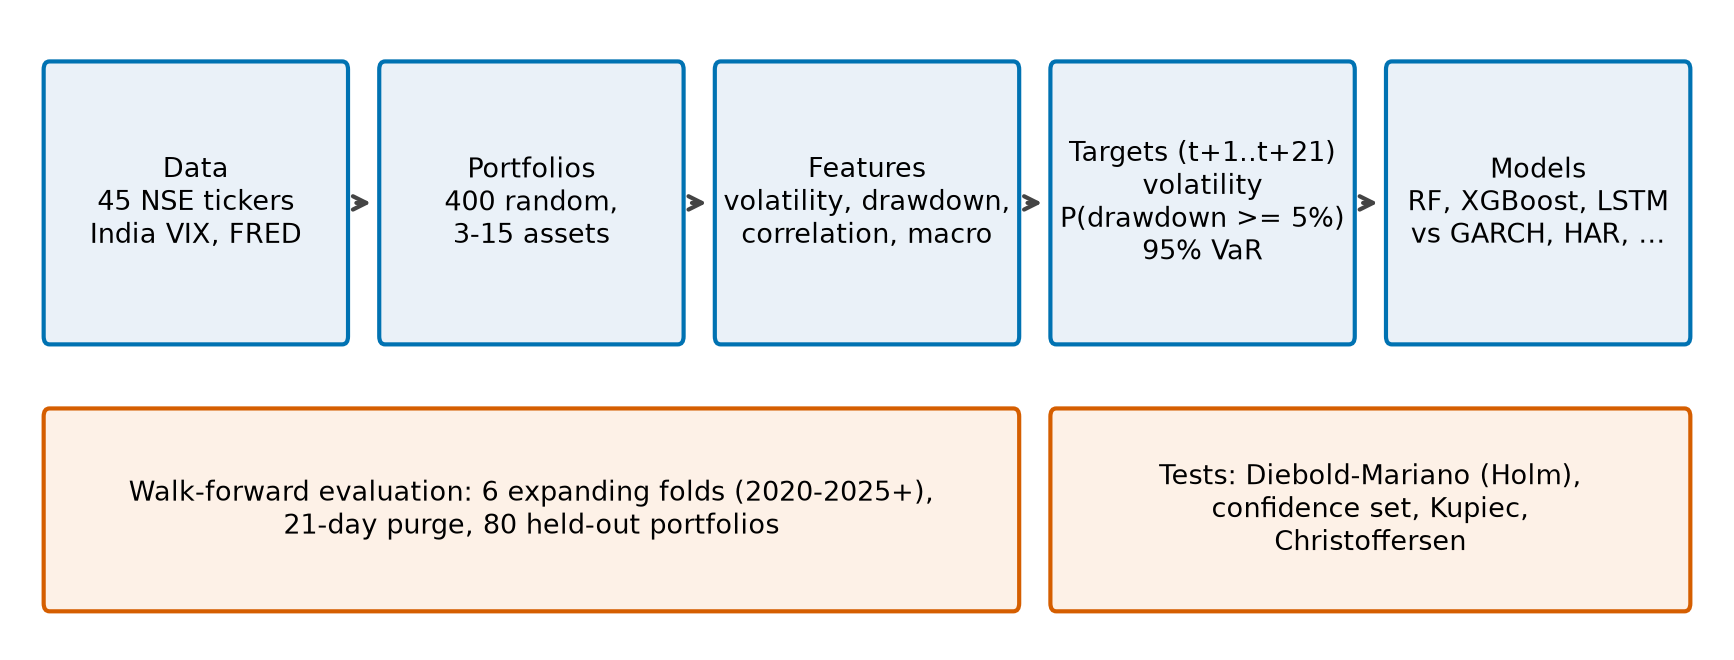
\includegraphics[width=0.92\textwidth]{figures/pipeline.png}
\caption{End-to-end pipeline and evaluation design.}
\label{fig:pipeline}
\end{figure*}

\section{Evaluation Protocol}
\textbf{Folds.} Six expanding-window folds test 2020, 2021, \dots, 2025 (the last runs to
September 2026), as in Fig.~\ref{fig:folds}. A training row is allowed only if its 21-day target
window ends before the test start (purge), and early stopping uses the last 252 training days.
After model selection, XGBoost and the LSTM are refit on all training rows for the chosen number of
rounds or epochs. Scalers are fit on training rows only. Every model, including each baseline, is
evaluated by one function on the same rows, and the run aborts if two models disagree on the row
index.

\begin{figure}[t]
\centering
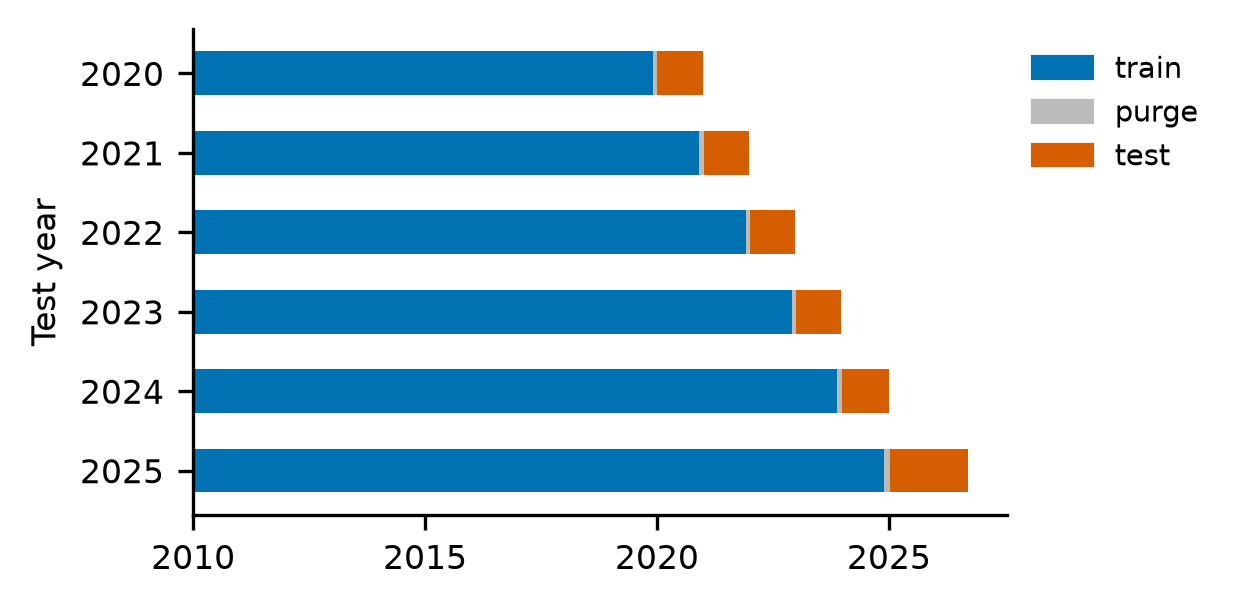
\includegraphics[width=0.78\columnwidth]{figures/folds.png}
\caption{Expanding-window folds with the purge between train and test.}
\label{fig:folds}
\end{figure}

\textbf{Metrics.} Volatility: QLIKE and MSE on variance (the consistent losses under a noisy proxy
\cite{patton2011}), plus RMSE, MAE and directional accuracy. Drawdown: Brier score, ROC-AUC, log
loss. VaR: pinball loss, exceedance rate, Kupiec test, Christoffersen independence and conditional
coverage tests per portfolio. We report mean $\pm$ standard deviation across folds.

\textbf{Significance.} Because portfolios share market days, tests use date-level losses averaged
over portfolios (about 330 dates), with a HAC variance for overlapping targets
\cite{dm1995,hln1997}. Holm's correction is applied within each pre-registered family; the
second-round choices (losses, families, combinations, regimes) were written into the code and pinned
by tests before any of those numbers existed. In total 119 inferential tests were run.

\textbf{Leakage controls.} Tests check that perturbing data after $t$ cannot change features,
baselines or backtests at $t$, that targets use only $t+1,\dots,t+H$, that purge gaps hold, and that
the deployed pipeline reproduces the evaluation predictions. There are 210 automated tests.

\section{Results}
\subsection{Volatility}
Table~\ref{tab:vol} and Fig.~\ref{fig:vol} show the ranking depends on the loss. On QLIKE,
GJR-GARCH-t is first (0.281) and the best ML model is the LSTM (0.299); on RMSE the combination of
HAR, GARCH and XGBoost is first (0.0697) with XGBoost second (0.0710). No ML model beats GJR
significantly (raw $p$ between 0.36 and 0.55 on QLIKE), while XGBoost and the LSTM beat naive
volatility on QLIKE (Holm-adjusted $p=0.015$ and $0.008$; Random Forest $0.074$,
Table~\ref{tab:dm}). On MSE-variance no ML model beats either reference. Fold-to-fold standard
deviations (about 0.05 on RMSE) exceed the gaps between the leading models, and the 90\% model
confidence set contains every model except naive under QLIKE. On held-out portfolios the picture is
the same (QLIKE: GJR 0.288, LSTM 0.305, XGBoost 0.312, naive 0.409).

\begin{table}[t]
\centering\small
\caption{Volatility forecasts, mean over six test years (lower is better except accuracy).}
\label{tab:vol}
\resizebox{\columnwidth}{!}{\begin{tabular}{lrrrr}
\hline
Model & QLIKE & MSE-var$\times10^3$ & RMSE & Dir.\ acc.\ (\%) \\
\hline
GJR-GARCH-t & 0.281 & 4.97 & 0.0734 & 66.7 \\
Combo HAR+GARCH+XGB & 0.298 & 5.29 & 0.0697 & 67.1 \\
LSTM & 0.299 & 5.18 & 0.0718 & 68.2 \\
XGBoost & 0.306 & 5.47 & 0.0710 & 66.9 \\
GARCH(1,1) & 0.309 & 5.27 & 0.0748 & 66.3 \\
Combo HAR+GARCH & 0.315 & 5.38 & 0.0717 & 66.7 \\
Random Forest & 0.338 & 5.80 & 0.0724 & 65.8 \\
EWMA & 0.345 & 6.72 & 0.0781 & 61.9 \\
HAR & 0.361 & 5.75 & 0.0728 & 65.6 \\
Naive & 0.399 & 8.21 & 0.0834 & -- \\
Ledoit-Wolf & 0.462 & 6.45 & 0.0834 & 63.1 \\
\hline
\end{tabular}
}
\end{table}

\begin{figure*}[t]
\centering
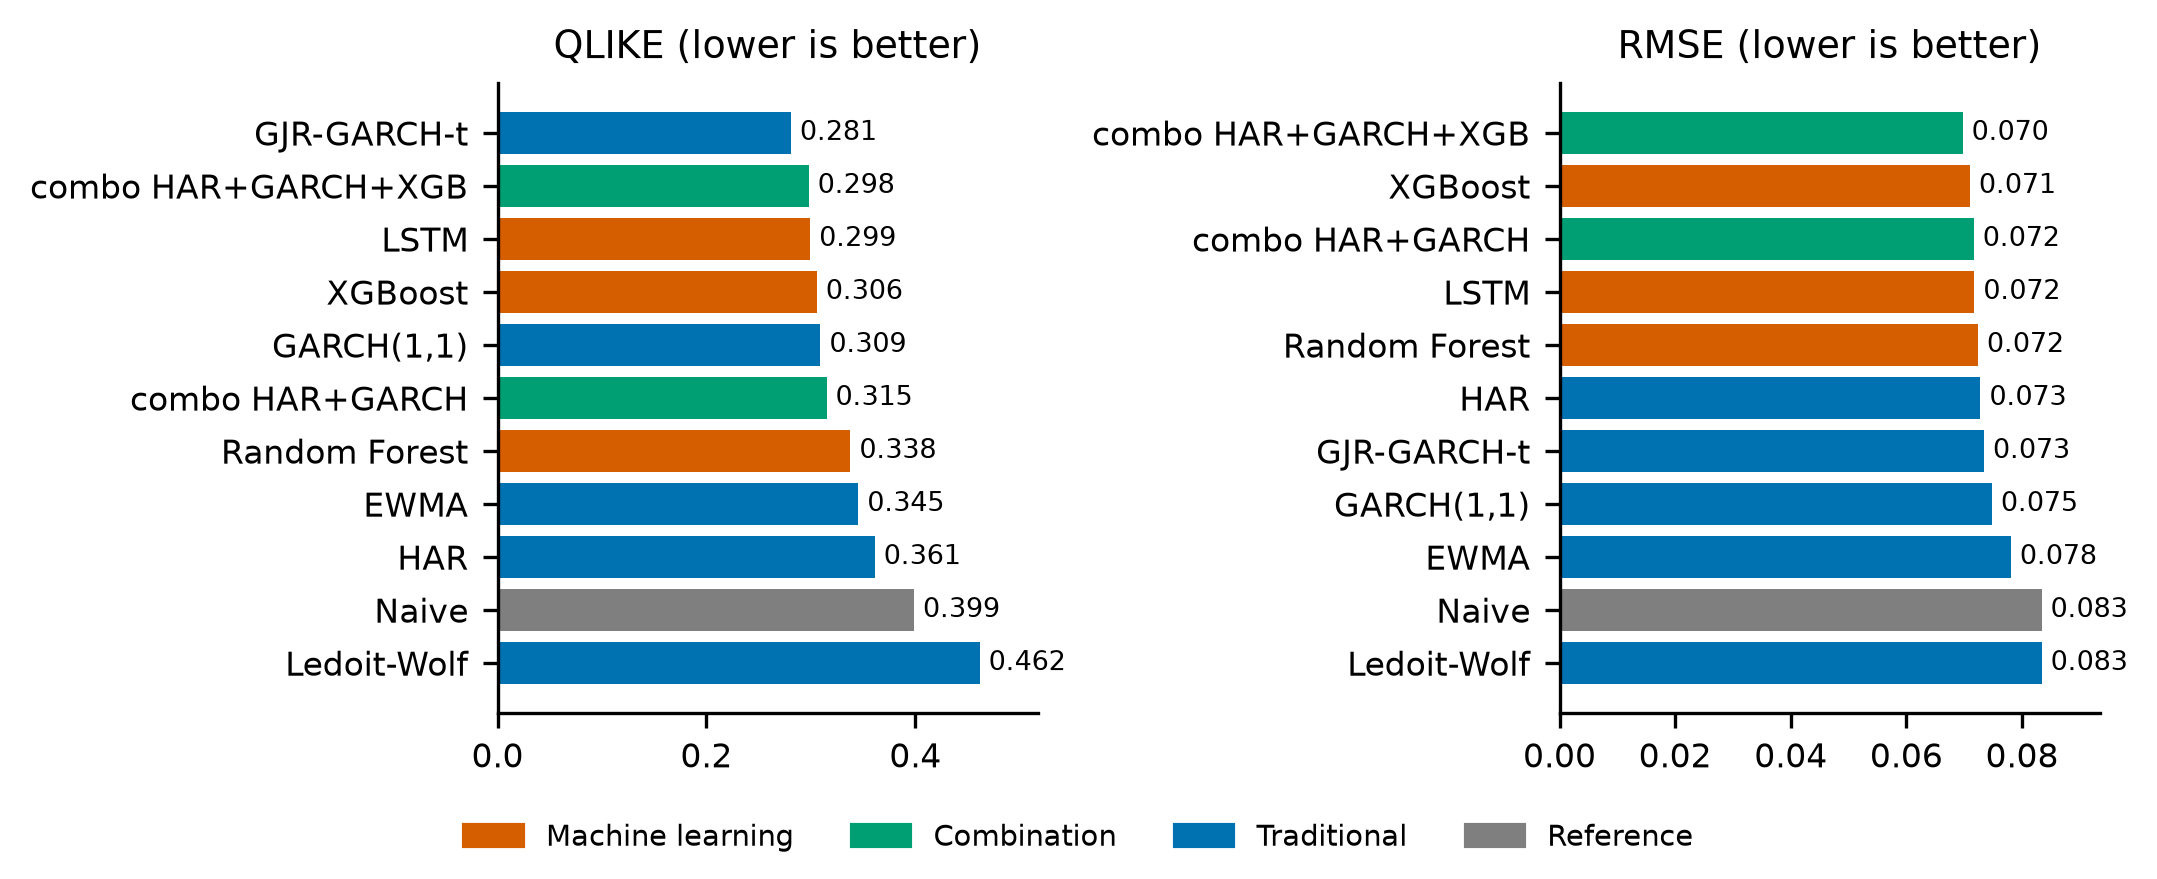
\includegraphics[width=0.88\textwidth]{figures/vol_bars.png}
\caption{Volatility ranking on QLIKE and RMSE (means over six folds).}
\label{fig:vol}
\end{figure*}

\begin{table}[t]
\centering\small
\caption{QLIKE differences of the ML models (Diebold-Mariano, ${\sim}$330 dates). Negative $\Delta$
favours the ML model.}
\label{tab:dm}
\resizebox{\columnwidth}{!}{\begin{tabular}{llrrr}
\hline
ML model & versus & $\Delta$ QLIKE & raw $p$ & Holm $p$ \\
\hline
Random Forest & best baseline (GJR) & +0.049 & 0.362 & 1.000 \\
Random Forest & naive & -0.063 & 0.007 & 0.074 \\
XGBoost & best baseline (GJR) & +0.020 & 0.531 & 1.000 \\
XGBoost & naive & -0.092 & 0.001 & 0.015 \\
LSTM & best baseline (GJR) & +0.017 & 0.548 & 1.000 \\
LSTM & naive & -0.095 & 0.001 & 0.008 \\
\hline
\end{tabular}
}
\end{table}

\begin{figure*}[t]
\centering
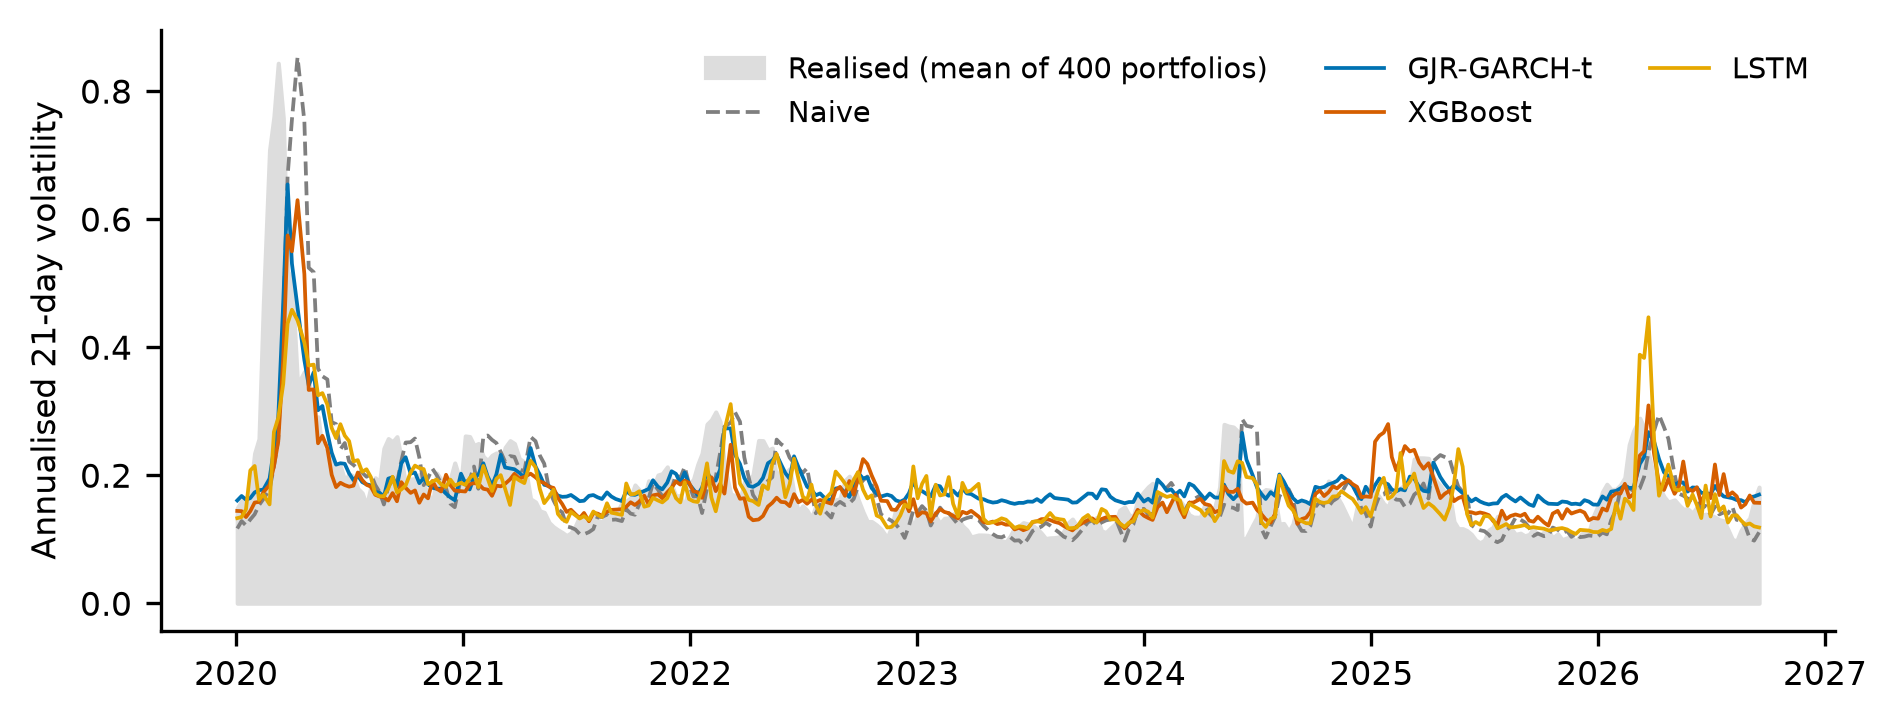
\includegraphics[width=0.92\textwidth]{figures/vol_time.png}
\caption{Mean predicted 21-day volatility across the 400 portfolios against the realised value
(the realised series is the outcome of the forecast made on the same date). The naive forecast lags
turning points; the others react earlier but also over- or under-shoot.}
\label{fig:voltime}
\end{figure*}

In calm periods (India VIX below its training median, 205 dates) XGBoost, the combination and HAR
lead (RMSE about 0.048--0.049); in stress (128 dates) GJR (0.108) and GARCH (0.113) lead, with the
LSTM at 0.114. No regime test is significant, and regimes are confounded with test year. Figure~\ref{fig:voltime}
shows how all models follow the 2020 spike and the smaller 2022 and 2026 episodes.

\subsection{Drawdown probability}
The simulated-drawdown model has the lowest Brier score (0.2046; Table~\ref{tab:dd}) and is well
calibrated overall (mean prediction 0.335 against a realised 0.318, whereas GARCH predicts 0.452).
Random Forest, LSTM and the combination are close (0.206--0.207); all beat the base rate (0.2199).
Its edge over GARCH (raw $p=0.034$) and the base rate (0.013) does not survive Holm correction
(0.101 and 0.052). GJR-GARCH has the best ROC-AUC (0.644), so it orders risky periods best even
though it over-predicts the level (mean 0.449). Figure~\ref{fig:dd} shows the calibration; the LSTM is the
least reliable at high predicted probabilities.

\begin{table}[t]
\centering\small
\caption{Drawdown ($\ge5\%$) probability, mean over six test years.}
\label{tab:dd}
\begin{tabular}{lrr}
\hline
Model & Brier & ROC-AUC \\
\hline
Simulated DD (recal.) & 0.2046 & 0.629 \\
Simulated DD & 0.2050 & 0.629 \\
Random Forest & 0.2061 & 0.607 \\
LSTM & 0.2062 & 0.632 \\
Combo HAR+GARCH+XGB & 0.2068 & 0.634 \\
XGBoost & 0.2101 & 0.616 \\
HAR & 0.2134 & 0.610 \\
Combo HAR+GARCH & 0.2144 & 0.626 \\
GJR-GARCH-t & 0.2196 & 0.643 \\
Base rate & 0.2199 & 0.500 \\
GARCH(1,1) & 0.2225 & 0.632 \\
Naive & 0.2229 & 0.615 \\
EWMA & 0.2237 & 0.614 \\
Ledoit-Wolf & 0.2420 & 0.588 \\
\hline
\end{tabular}

\end{table}

\begin{figure}[t]
\centering
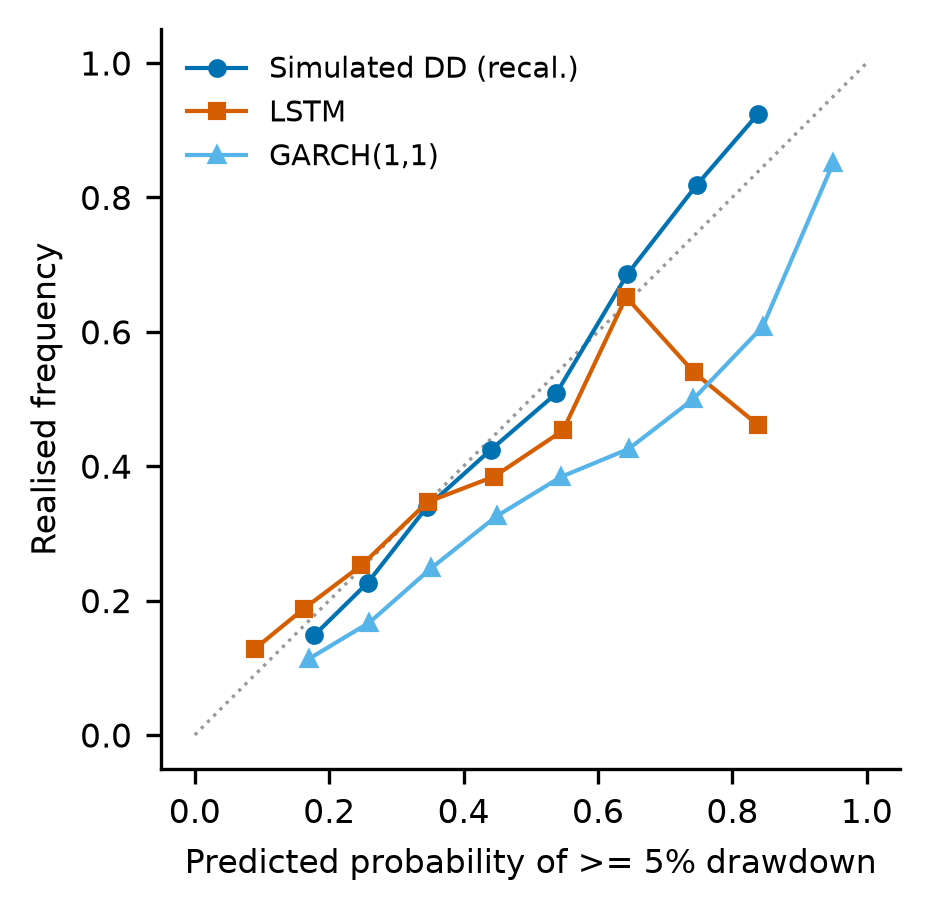
\includegraphics[width=0.78\columnwidth]{figures/dd_reliability.png}
\caption{Reliability of the drawdown probability (bins with more than 200 rows).}
\label{fig:dd}
\end{figure}

\subsection{Value-at-Risk}
Pinball losses differ only in the fourth decimal (Table~\ref{tab:var}), with GJR-GARCH-t lowest
(1.367$\times10^{-3}$). Average exceedance is 4.6--6.0\% for most models, but the yearly rate ranges
from about 2\% to 11\% (Fig.~\ref{fig:var}): the GARCH-type models under-state risk in 2020--21 (exceedance 7--8\%)
and over-state it in 2023--25 (2--3\%). The pooled Kupiec test rejects 5\% coverage in most years, but it treats
about 20,000 dependent portfolio-dates a year as independent; a date-clustered test does not reject
the average rate for any model. Christoffersen's independence test rejects for 1--3\% of portfolios
for most models (6\% for the LSTM, against 49\% before the HAR/GARCH inputs). The conformal
correction brings average exceedance to 4.6--4.9\% and narrows the yearly range, with unchanged or
slightly worse pinball loss. For expected shortfall (baselines only) GJR and filtered historical
simulation come closest to the realised tail size (ratio 1.02--1.03), whereas for the normal-based models
the realised tail loss is 12--14\% larger than predicted.

\begin{table}[t]
\centering\small
\caption{95\% one-day VaR. ``Exc.'' is the mean exceedance rate; ``Kupiec rej.'' counts test years
with a pooled rejection; (cal.) is after conformal calibration.}
\label{tab:var}
\resizebox{\columnwidth}{!}{\begin{tabular}{lrrrr}
\hline
Model & Pinball$\times10^3$ & Exc.\ (\%) & Yearly range (\%) & Kupiec rej. \\
\hline
GJR-GARCH-t & 1.367 & 4.7 & 2.0--8.1 & 5/6 \\
Combo HAR+GARCH+XGB & 1.384 & 5.0 & 2.3--8.2 & 5/6 \\
GARCH(1,1) & 1.392 & 4.6 & 2.0--8.1 & 5/6 \\
Filtered hist. sim. & 1.394 & 5.3 & 2.4--8.9 & 6/6 \\
XGBoost & 1.411 & 5.8 & 3.0--8.4 & 6/6 \\
Naive & 1.406 & 6.0 & 2.8--8.8 & 6/6 \\
LSTM & 1.457 & 5.6 & 2.3--10.7 & 6/6 \\
Historical VaR & 1.479 & 5.9 & 3.8--11.1 & 6/6 \\
GJR-GARCH-t (cal.) & 1.371 & 4.6 & 2.9--7.2 & 4/6 \\
XGBoost (cal.) & 1.436 & 4.8 & 2.6--7.6 & 6/6 \\
LSTM (cal.) & 1.446 & 4.9 & 2.3--7.8 & 5/6 \\
\hline
\end{tabular}
}
\end{table}

\begin{figure}[t]
\centering
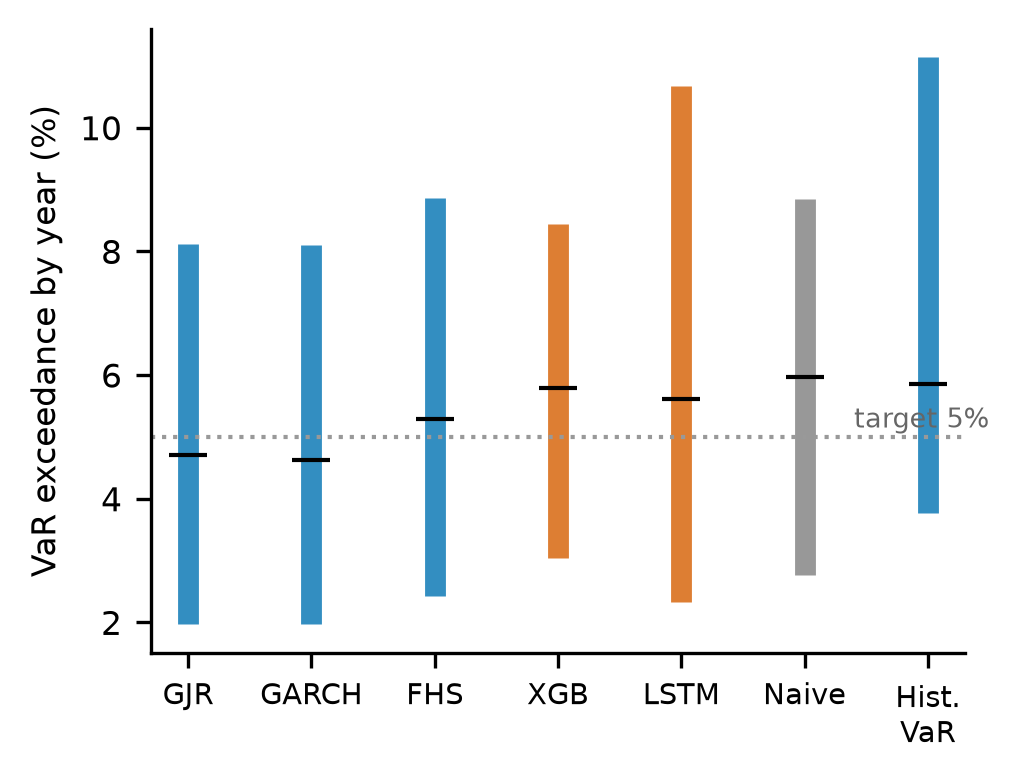
\includegraphics[width=0.78\columnwidth]{figures/var_yearly.png}
\caption{Range of the yearly VaR exceedance rate (bar) and its mean (tick).}
\label{fig:var}
\end{figure}

\subsection{Effect of model-based inputs}\label{sec:r4}
Adding the HAR and GARCH forecasts as inputs improved most ML metrics: LSTM QLIKE 0.321 to 0.299,
XGBoost 0.317 to 0.306, drawdown AUC 0.606 to 0.632 (LSTM) and 0.584 to 0.616 (XGBoost). None of
the eight paired tests is significant (raw $p$ 0.13--0.63), so we treat this as suggestive. It is
consistent with ML working best as a complement to, not a replacement for, econometric models.

\subsection{Downstream test: volatility targeting}
To see whether the forecasts matter in use, each model's 21-day volatility forecast sets the
exposure to the portfolio, $\min(1, 10\%/\hat\sigma)$, with the rest in cash at 6\% a year,
rebalanced on every forecast date (weekly), buy-and-hold in between, no leverage, and 15 basis
points of cost charged on the change from the drifted position. The portfolios themselves are the
constant-weight series (their internal turnover is not charged). The main measure is the RMSE
between the realised volatility of non-overlapping 63-day blocks and the 10\% target, over blocks
where the target is reachable without leverage; this metric was fixed after a code review of a
first version and is not part of the pre-registered set.

Table~\ref{tab:down} and Fig.~\ref{fig:down} show that any forecast brings realised volatility to
about 10--11\% against 19\% unscaled, and roughly halves the maximum drawdown (from $-17.4\%$ to
$-8$ to $-10\%$). Differences between forecasts are small (0.0175--0.0218, except HAR and
Ledoit-Wolf) and smaller than the fold-to-fold spread. EWMA, naive and GJR rank first; the combination
and ML models are close behind, not ahead. The Diebold-Mariano test on the date-level 21-day
tracking loss favours the HAR+GARCH+XGBoost combination over naive (Holm $p=0.0006$; $0.0003$ on
held-out portfolios) and EWMA and GARCH over naive (Holm about 0.04--0.05), but no model beats
GJR (smallest raw $p$ 0.13). The two views disagree on the combination, so no ranking is robust.
Sharpe ratios (0.65--0.74) are indistinguishable. In short, forecasts matter versus not using one,
but ML adds no reliable edge over the simple baselines here either.

\begin{table}[t]
\centering\small
\caption{Volatility-targeted portfolios (target 10\%), mean over six folds, 400 portfolios.
Track.\ err.\ is the RMSE of 63-day realised volatility versus the target on reachable blocks.}
\label{tab:down}
\resizebox{\columnwidth}{!}{\begin{tabular}{lrrrrr}
\hline
Sizing forecast & Track.\ err. & Vol (\%) & Sharpe & Max DD (\%) & Turn.\ /yr \\
\hline
Oracle (ceiling) & 0.0046 & 9.9 & 1.22 & -6.9 & 3.2 \\
EWMA & 0.0175 & 10.6 & 0.65 & -9.5 & 2.5 \\
Naive & 0.0187 & 11.0 & 0.67 & -9.8 & 3.1 \\
GJR-GARCH-t & 0.0192 & 9.7 & 0.74 & -8.4 & 1.8 \\
LSTM & 0.0195 & 10.6 & 0.68 & -9.6 & 3.1 \\
Combo HAR+GARCH+XGB & 0.0204 & 10.3 & 0.71 & -9.4 & 1.6 \\
GARCH(1,1) & 0.0210 & 9.7 & 0.72 & -8.7 & 1.6 \\
Random Forest & 0.0212 & 10.9 & 0.70 & -9.7 & 2.3 \\
Combo HAR+GARCH & 0.0214 & 10.2 & 0.70 & -9.3 & 1.5 \\
XGBoost & 0.0218 & 10.8 & 0.71 & -9.7 & 2.4 \\
HAR & 0.0246 & 10.9 & 0.67 & -10.2 & 1.6 \\
Ledoit-Wolf & 0.0361 & 10.7 & 0.66 & -10.3 & 0.3 \\
No scaling & 0.1076 & 19.3 & 0.77 & -17.4 & 0.0 \\
\hline
\end{tabular}
}
\end{table}

\begin{figure}[t]
\centering
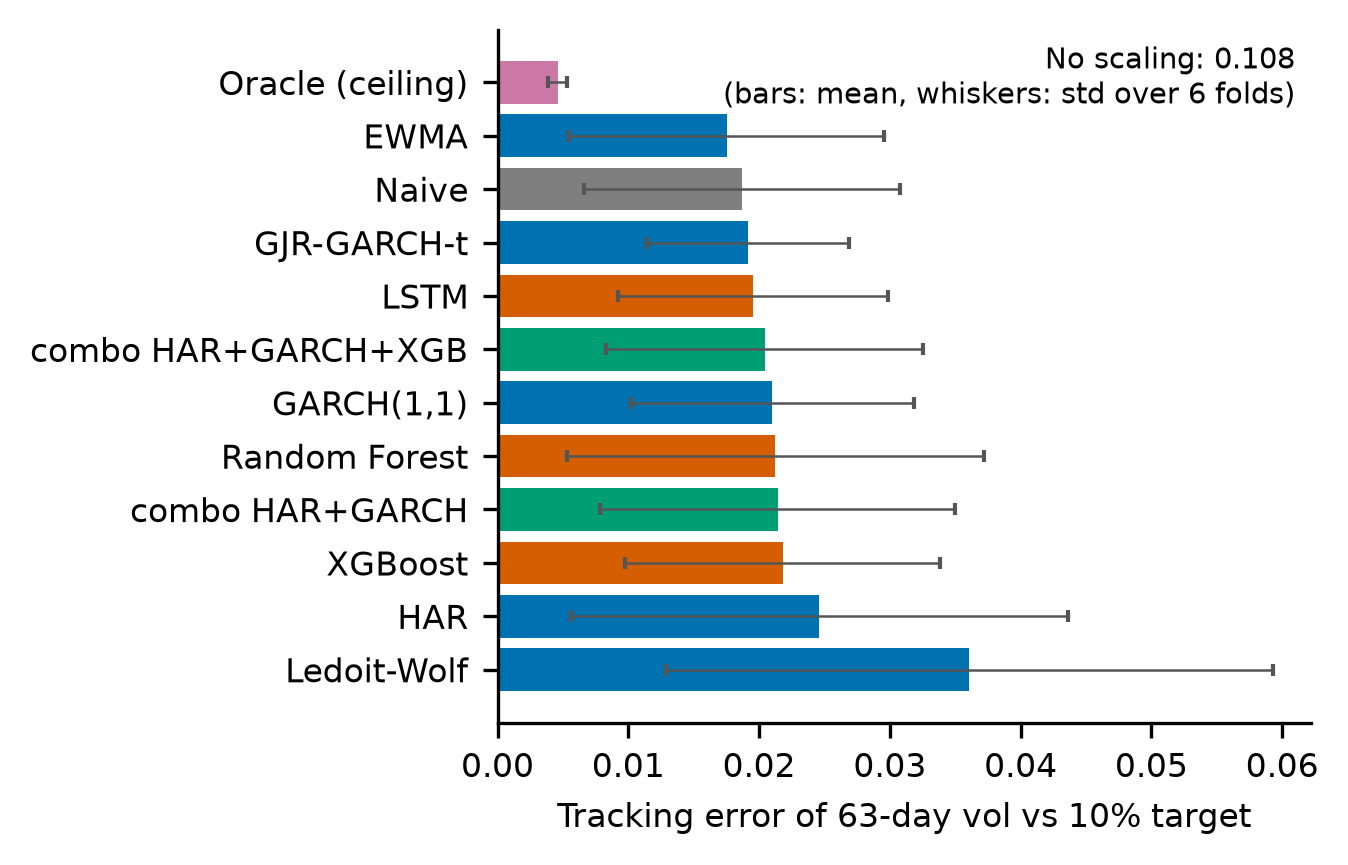
\includegraphics[width=0.9\columnwidth]{figures/downstream.png}
\caption{Tracking error by sizing forecast (whiskers: standard deviation over folds).}
\label{fig:down}
\end{figure}

\section{Discussion}
\textbf{Where ML helps.} Against naive volatility, XGBoost and the LSTM win significantly on QLIKE,
and in calm regimes the tree models lead. Combining HAR, GARCH and XGBoost gives the lowest RMSE and
the most stable results across measures. \textbf{Where it does not.} No ML model significantly
beats GJR-GARCH-t after correction, the LSTM and tree models are less reliable on VaR clustering
and drawdown calibration, and the downstream test shows no reliable gain. This echoes the
finding that leverage-aware GARCH models are hard to beat \cite{hansen2005}. \textbf{Why the comparison is
fragile.} Only about 190 independent 21-day periods exist since 2010, portfolios share market days
so 400 portfolios add little independent information, and several rankings change with the loss.
We therefore emphasise paired tests, the model confidence set (which cannot separate most models)
and held-out portfolios over point rankings.

\textbf{Limitations.} (i) Hyperparameters were not tuned and only one seed per model was used in
the final configuration; in an earlier configuration seeds moved the LSTM noticeably (volatility RMSE
0.070--0.075) while XGBoost and Random Forest barely moved. (ii) Yahoo data are delayed and
sometimes wrong, today's large caps imply survivorship bias, no bond asset is included (Indian gilt
ETFs lack history to 2010) and the macro series are US-based. (iii) Portfolios are rebalanced daily,
which is not how investors hold them. (iv) The date-level dynamic-quantile test is oversized in our
simulations and is reported only as descriptive. (v) The DM, confidence-set and coverage tests
assume stationary loss differences, which expanding windows do not guarantee. (vi) Some choices,
such as the combination members, were made after seeing earlier ranks. (vii) The deployed models
used in the app are weakly trained (for example the LSTM stops after one epoch for two heads), so
they serve the demonstration, while every reported number comes from the walk-forward fold models.
This is an educational project and not investment advice.

\section{Conclusion}
On 45 Indian stocks and ETFs, ML models predict portfolio risk about as well as strong econometric
models, and better than naive persistence, but not significantly better than GJR-GARCH with
$t$ errors. The most dependable improvements come from combining ML with HAR and GARCH forecasts
and from simulating drawdowns from a fitted volatility model. A downstream volatility-targeting test
confirms that using any forecast brings realised risk close to target, without separating the models.
Future work includes tuning and multiple seeds with the new inputs, other horizons and assets (bonds,
international equities), an ES head for the ML models, and regime-aware training. All code, tests,
tables and the dashboard are in the project repository.

\begin{thebibliography}{99}
\bibitem{bollerslev1986} T. Bollerslev, ``Generalized autoregressive conditional heteroskedasticity,'' \emph{J. Econometrics}, vol.~31, no.~3, pp.~307--327, 1986.
\bibitem{glosten1993} L. R. Glosten, R. Jagannathan, D. E. Runkle, ``On the relation between the expected value and the volatility of the nominal excess return on stocks,'' \emph{J. Finance}, vol.~48, no.~5, pp.~1779--1801, 1993.
\bibitem{riskmetrics1996} J.P. Morgan/Reuters, \emph{RiskMetrics---Technical Document}, 4th ed., 1996.
\bibitem{corsi2009} F. Corsi, ``A simple approximate long-memory model of realized volatility,'' \emph{J. Financial Econometrics}, vol.~7, no.~2, pp.~174--196, 2009.
\bibitem{hansen2005} P. R. Hansen, A. Lunde, ``A forecast comparison of volatility models: does anything beat a GARCH(1,1)?'' \emph{J. Applied Econometrics}, vol.~20, no.~7, pp.~873--889, 2005.
\bibitem{christensen2023} K. Christensen, M. Siggaard, B. Veliyev, ``A machine learning approach to volatility forecasting,'' \emph{J. Financial Econometrics}, vol.~21, no.~5, pp.~1680--1727, 2023.
\bibitem{gu2020} S. Gu, B. Kelly, D. Xiu, ``Empirical asset pricing via machine learning,'' \emph{Rev. Financial Studies}, vol.~33, no.~5, pp.~2223--2273, 2020.
\bibitem{breiman2001} L. Breiman, ``Random forests,'' \emph{Machine Learning}, vol.~45, pp.~5--32, 2001.
\bibitem{chen2016} T. Chen, C. Guestrin, ``XGBoost: a scalable tree boosting system,'' in \emph{Proc. KDD}, 2016, pp.~785--794.
\bibitem{hochreiter1997} S. Hochreiter, J. Schmidhuber, ``Long short-term memory,'' \emph{Neural Computation}, vol.~9, no.~8, pp.~1735--1780, 1997.
\bibitem{patton2011} A. J. Patton, ``Volatility forecast comparison using imperfect volatility proxies,'' \emph{J. Econometrics}, vol.~160, no.~1, pp.~246--256, 2011.
\bibitem{dm1995} F. X. Diebold, R. S. Mariano, ``Comparing predictive accuracy,'' \emph{J. Business \& Economic Statistics}, vol.~13, no.~3, pp.~253--263, 1995.
\bibitem{hln1997} D. Harvey, S. Leybourne, P. Newbold, ``Testing the equality of prediction mean squared errors,'' \emph{Int. J. Forecasting}, vol.~13, no.~2, pp.~281--291, 1997.
\bibitem{holm1979} S. Holm, ``A simple sequentially rejective multiple test procedure,'' \emph{Scandinavian J. Statistics}, vol.~6, no.~2, pp.~65--70, 1979.
\bibitem{hansen2011} P. R. Hansen, A. Lunde, J. M. Nason, ``The model confidence set,'' \emph{Econometrica}, vol.~79, no.~2, pp.~453--497, 2011.
\bibitem{kupiec1995} P. H. Kupiec, ``Techniques for verifying the accuracy of risk measurement models,'' \emph{J. Derivatives}, vol.~3, no.~2, pp.~73--84, 1995.
\bibitem{christoffersen1998} P. F. Christoffersen, ``Evaluating interval forecasts,'' \emph{Int. Economic Review}, vol.~39, no.~4, pp.~841--862, 1998.
\bibitem{fissler2016} T. Fissler, J. F. Ziegel, ``Higher order elicitability and Osband's principle,'' \emph{Annals of Statistics}, vol.~44, no.~4, pp.~1680--1707, 2016.
\bibitem{patton2019} A. J. Patton, J. F. Ziegel, R. Chen, ``Dynamic semiparametric models for expected shortfall (and Value-at-Risk),'' \emph{J. Econometrics}, vol.~211, no.~2, pp.~388--413, 2019.
\bibitem{koenker1978} R. Koenker, G. Bassett, ``Regression quantiles,'' \emph{Econometrica}, vol.~46, no.~1, pp.~33--50, 1978.
\bibitem{barone1999} G. Barone-Adesi, K. Giannopoulos, L. Vosper, ``VaR without correlations for portfolios of derivative securities,'' \emph{J. Futures Markets}, vol.~19, no.~5, pp.~583--602, 1999.
\bibitem{gibbs2021} I. Gibbs, E. Cand\`es, ``Adaptive conformal inference under distribution shift,'' in \emph{Proc. NeurIPS}, 2021.
\bibitem{ledoit2004} O. Ledoit, M. Wolf, ``A well-conditioned estimator for large-dimensional covariance matrices,'' \emph{J. Multivariate Analysis}, vol.~88, no.~2, pp.~365--411, 2004.
\bibitem{moreira2017} A. Moreira, T. Muir, ``Volatility-managed portfolios,'' \emph{J. Finance}, vol.~72, no.~4, pp.~1611--1644, 2017.
\end{thebibliography}

\end{document}
